% High level block diagram of the ethrc motor controller PCB.
% Build: pdflatex block_diagram.tex && pdftocairo -png -r 300 -singlefile block_diagram.pdf block_diagram
% The figure is drawn at its printed size (1:1 on the A3 "Block Diagram" schematic page).
\documentclass[tikz,border=4mm]{standalone}
\usepackage[T1]{fontenc}
\usepackage{helvet}
\renewcommand{\familydefault}{\sfdefault}
\usetikzlibrary{arrows.meta,calc,fit,backgrounds}

\definecolor{extfill}{HTML}{FFD8A8}   % external parts (orange)
\definecolor{extline}{HTML}{E8590C}
\definecolor{intfill}{HTML}{D0EBFF}   % PCB components (light blue)
\definecolor{intline}{HTML}{1C7ED6}
\definecolor{connfill}{HTML}{1864AB}  % PCB connectors (dark blue)
\definecolor{pwr}{HTML}{C92A2A}       % power
\definecolor{sig}{HTML}{343A40}       % signals

\tikzset{
  >={Stealth[length=3mm,width=2mm]},
  blk/.style={draw=intline, fill=intfill, line width=0.6pt, rounded corners=1.5mm, align=center,
              minimum height=1.9cm, text width=#1, inner sep=2mm},
  blk/.default=4.6cm,
  ext/.style={draw=extline, fill=extfill, line width=0.6pt, rounded corners=1.5mm, align=center,
              minimum height=1.5cm, text width=3.4cm, inner sep=2mm},
  conn/.style={draw=connfill, fill=connfill, text=white, line width=0.6pt, align=center,
               minimum height=1.1cm, text width=2.6cm, inner sep=1.5mm, font=\small\bfseries},
  dnp/.style={dashed},
  sigb/.style={draw=sig, line width=0.8pt, <->},
  sigr/.style={draw=sig, line width=0.8pt, ->},
  pwrl/.style={draw=pwr, line width=2pt, ->},
  pwrn/.style={draw=pwr, line width=2pt},
  lab/.style={font=\small, fill=white, inner sep=1pt, align=center},
  plab/.style={font=\small\bfseries, text=pwr, fill=white, inner sep=1pt, align=center},
}
\newcommand{\rail}[1]{{\footnotesize\itshape\color{pwr}#1}}

\begin{document}
\hyphenpenalty=10000\exhyphenpenalty=10000
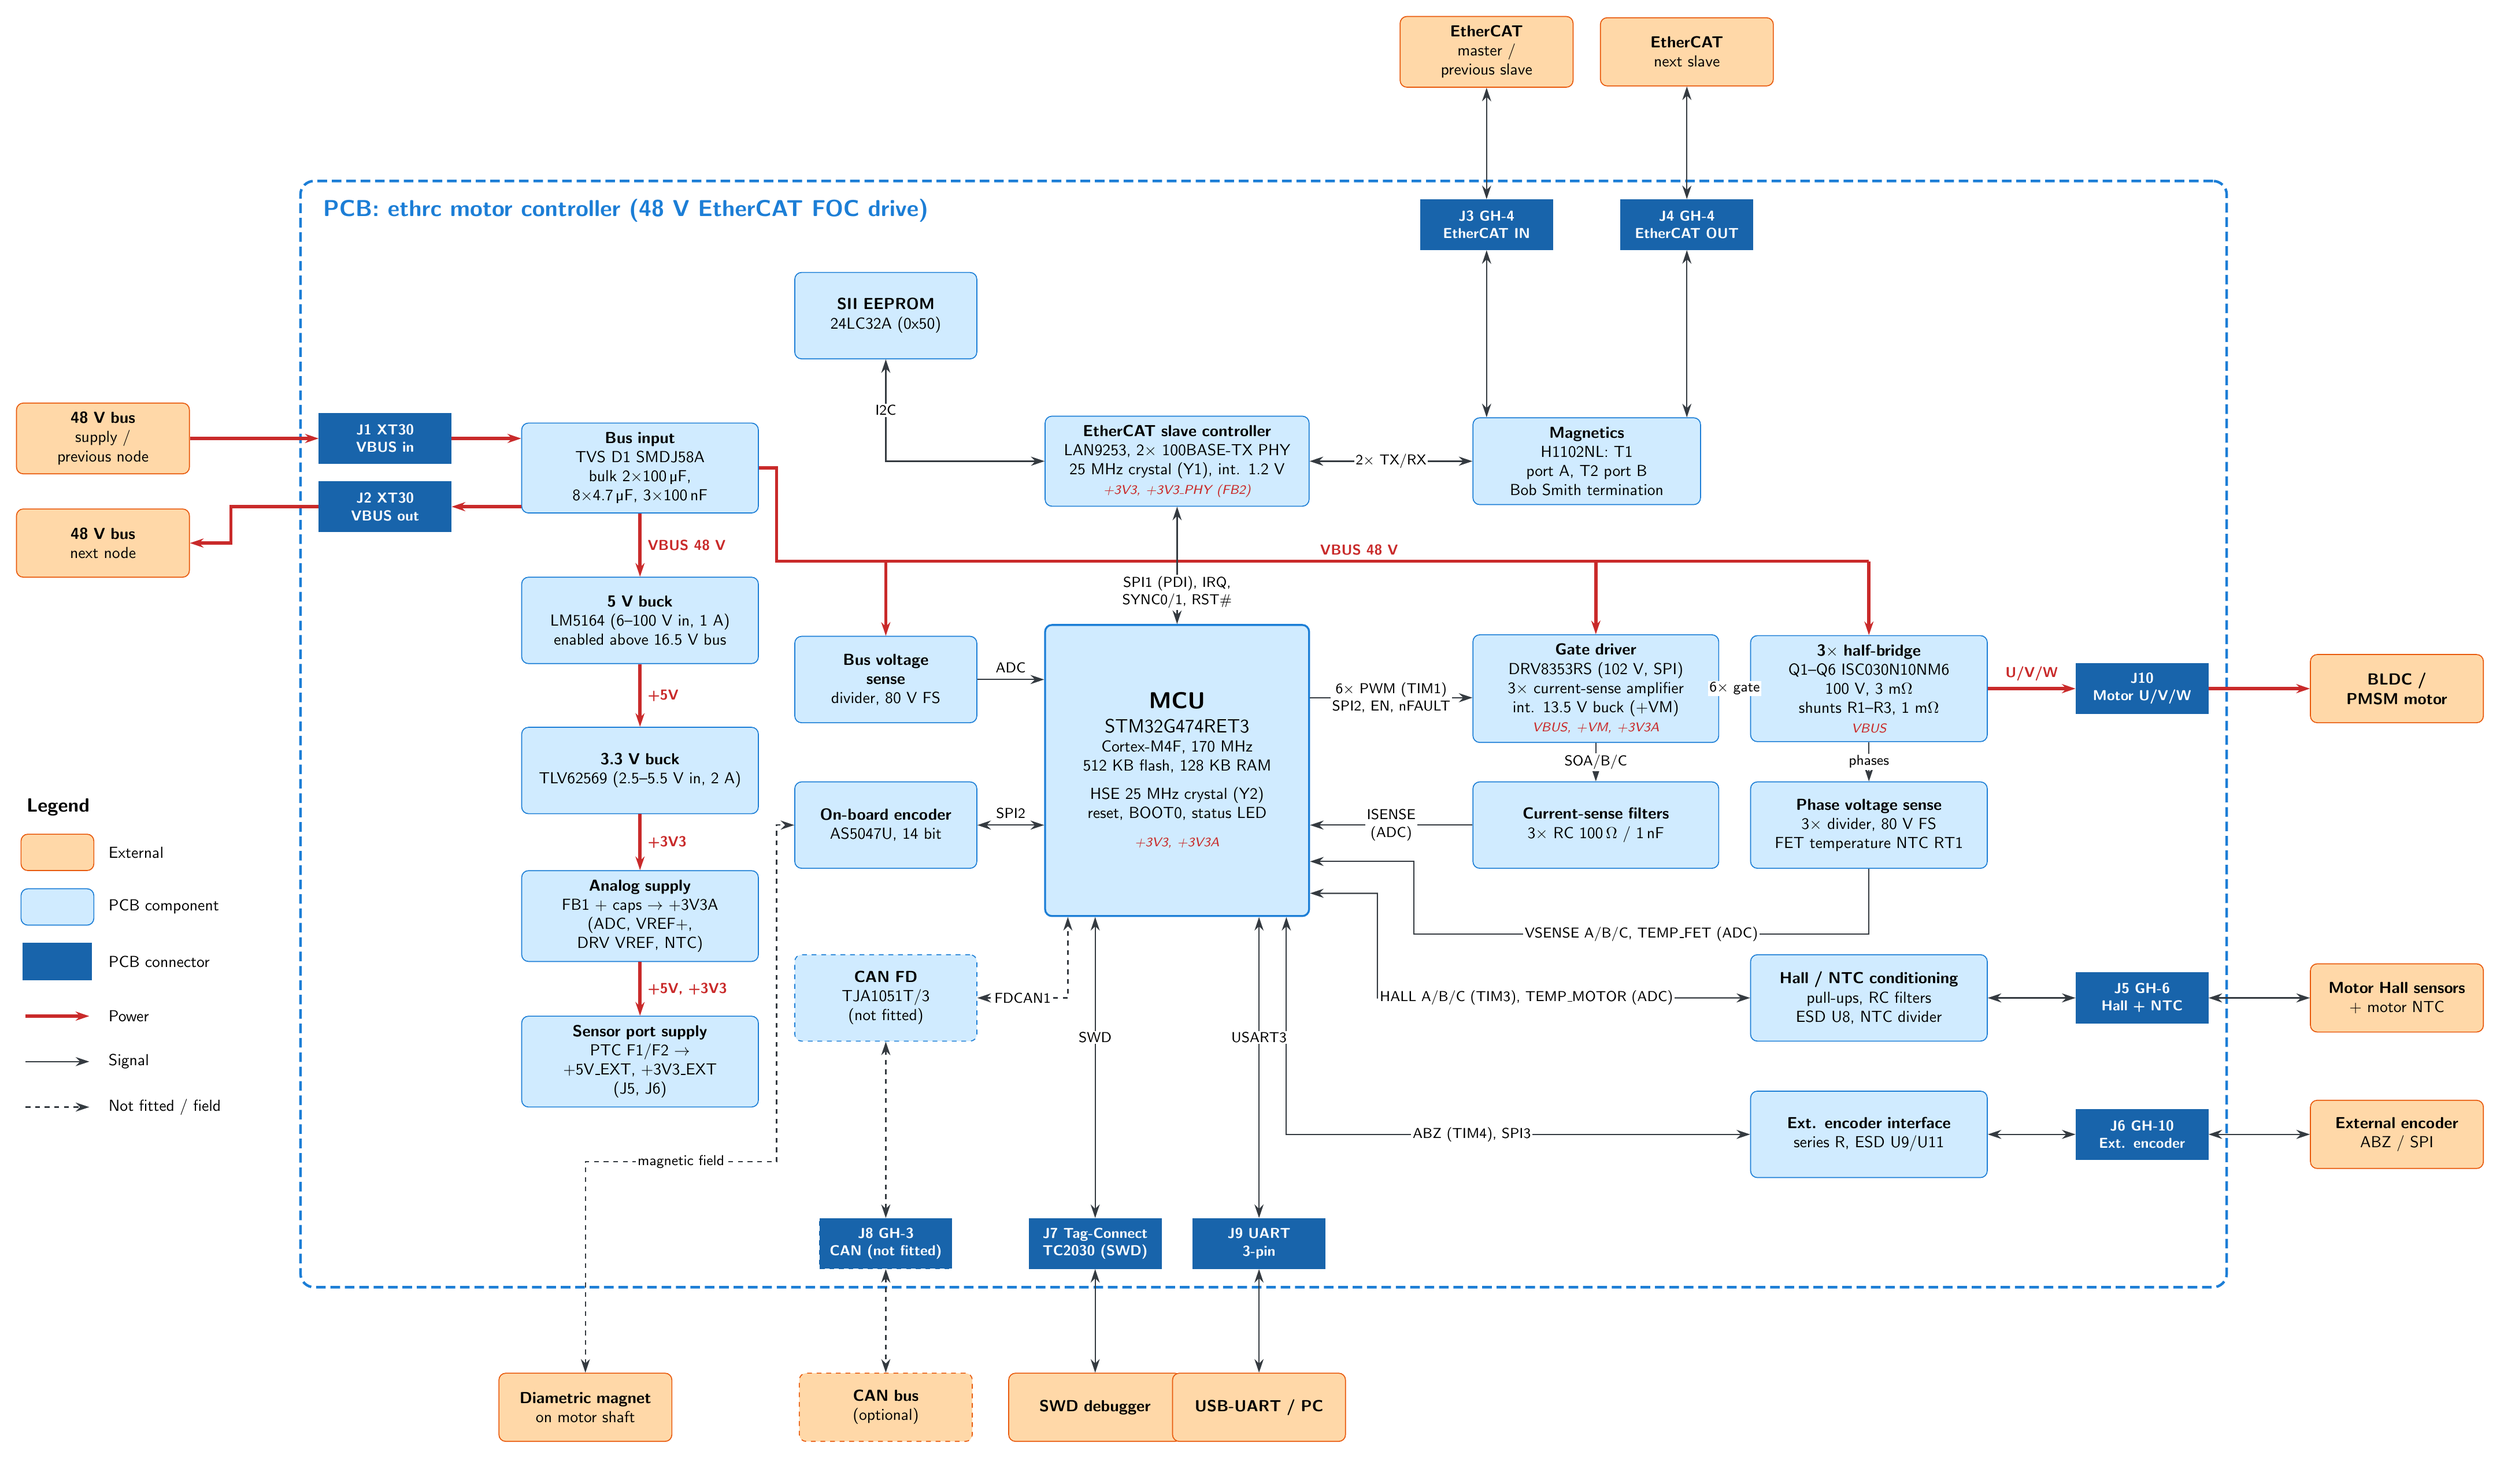
\begin{tikzpicture}

% ------------------------------------------------------------ power column
\node[blk=4.8cm] (prot) at (8.2,15.25)
  {\textbf{Bus input}\\TVS D1 SMDJ58A\\bulk 2$\times$100\,\textmu F, 8$\times$4.7\,\textmu F, 3$\times$100\,nF};
\node[blk=4.8cm] (buck5) at (8.2,11.9)
  {\textbf{5 V buck}\\LM5164 (6--100 V in, 1 A)\\enabled above 16.5 V bus};
\node[blk=4.8cm] (buck3) at (8.2,8.6)
  {\textbf{3.3 V buck}\\TLV62569 (2.5--5.5 V in, 2 A)};
\node[blk=4.8cm] (ana) at (8.2,5.4)
  {\textbf{Analog supply}\\FB1 + caps $\rightarrow$ +3V3A\\(ADC, VREF+, DRV VREF, NTC)};
\node[blk=4.8cm] (ptc) at (8.2,2.2)
  {\textbf{Sensor port supply}\\PTC F1/F2 $\rightarrow$ +5V\_EXT, +3V3\_EXT\\(J5, J6)};

% ------------------------------------------------------------ middle column
\node[blk=3.6cm] (eep) at (13.6,18.6) {\textbf{SII EEPROM}\\24LC32A (0x50)};
\node[blk=3.6cm] (vbsen) at (13.6,10.6) {\textbf{Bus voltage}\\\textbf{sense}\\divider, 80 V FS};
\node[blk=3.6cm] (enc) at (13.6,7.4) {\textbf{On-board encoder}\\AS5047U, 14 bit};
\node[blk=3.6cm, dnp] (can) at (13.6,3.6) {\textbf{CAN FD}\\TJA1051T/3\\(not fitted)};

% ------------------------------------------------------------ MCU and EtherCAT
\node[blk=5.4cm, minimum height=6.4cm, line width=1.2pt] (mcu) at (20.0,8.6)
  {{\Large\textbf{MCU}}\\[1mm]{\large STM32G474RET3}\\Cortex-M4F, 170 MHz\\512 KB flash, 128 KB RAM\\[2mm]
   HSE 25 MHz crystal (Y2)\\reset, BOOT0, status LED\\[2mm]\rail{+3V3, +3V3A}};
\node[blk=5.4cm] (esc) at (20.0,15.4)
  {\textbf{EtherCAT slave controller}\\LAN9253, 2$\times$ 100BASE-TX PHY\\25 MHz crystal (Y1), int. 1.2 V\\\rail{+3V3, +3V3\_PHY (FB2)}};
\node[blk=4.6cm] (mag) at (29.0,15.4) {\textbf{Magnetics}\\H1102NL: T1 port A, T2 port B\\Bob Smith termination};

% ------------------------------------------------------------ motor drive
\node[blk=5.0cm] (drv) at (29.2,10.4)
  {\textbf{Gate driver}\\DRV8353RS (102 V, SPI)\\3$\times$ current-sense amplifier\\int. 13.5 V buck (+VM)\\\rail{VBUS, +VM, +3V3A}};
\node[blk=4.8cm] (bridge) at (35.2,10.4)
  {\textbf{3$\times$ half-bridge}\\Q1--Q6 ISC030N10NM6\\100 V, 3 m\(\Omega\)\\shunts R1--R3, 1 m\(\Omega\)\\\rail{VBUS}};
\node[blk=5.0cm] (isen) at (29.2,7.4) {\textbf{Current-sense filters}\\3$\times$ RC 100\,\(\Omega\) / 1\,nF};
\node[blk=4.8cm] (vsen) at (35.2,7.4) {\textbf{Phase voltage sense}\\3$\times$ divider, 80 V FS\\FET temperature NTC RT1};

% ------------------------------------------------------------ sensor ports
\node[blk=4.8cm] (hall) at (35.2,3.6) {\textbf{Hall / NTC conditioning}\\pull-ups, RC filters\\ESD U8, NTC divider};
\node[blk=4.8cm] (extc) at (35.2,0.6) {\textbf{Ext. encoder interface}\\series R, ESD U9/U11};

% ------------------------------------------------------------ connectors
\node[conn] (j1) at (2.6,15.9) {J1 XT30\\VBUS in};
\node[conn] (j2) at (2.6,14.4) {J2 XT30\\VBUS out};
\node[conn] (j3) at (26.8,20.6) {J3 GH-4\\EtherCAT IN};
\node[conn] (j4) at (31.2,20.6) {J4 GH-4\\EtherCAT OUT};
\node[conn] (j10) at (41.2,10.4) {J10\\Motor U/V/W};
\node[conn] (j5) at (41.2,3.6) {J5 GH-6\\Hall + NTC};
\node[conn] (j6) at (41.2,0.6) {J6 GH-10\\Ext. encoder};
\node[conn, dnp] (j8) at (13.6,-1.8) {J8 GH-3\\CAN (not fitted)};
\node[conn] (j7) at (18.2,-1.8) {J7 Tag-Connect\\TC2030 (SWD)};
\node[conn] (j9) at (21.8,-1.8) {J9 UART\\3-pin};

% ------------------------------------------------------------ PCB outline
\begin{scope}[on background layer]
  \node[draw=intline, line width=1.6pt, dash pattern=on 6pt off 3pt, rounded corners=3mm,
        fit=(j1)(j2)(j3)(j4)(j10)(j5)(j6)(j7)(j8)(j9)(eep)(ptc), inner sep=4mm] (pcb) {};
\end{scope}
\node[anchor=north west, font=\Large\bfseries, text=intline] at ($(pcb.north west)+(4mm,-3mm)$)
  {PCB: ethrc motor controller (48 V EtherCAT FOC drive)};

% ------------------------------------------------------------ external parts
\node[ext] (bus) at (-3.6,15.9) {\textbf{48 V bus}\\supply /\\previous node};
\node[ext] (busn) at (-3.6,13.6) {\textbf{48 V bus}\\next node};
\node[ext] (master) at (26.8,24.4) {\textbf{EtherCAT}\\master /\\previous slave};
\node[ext] (next) at (31.2,24.4) {\textbf{EtherCAT}\\next slave};
\node[ext] (motor) at (46.8,10.4) {\textbf{BLDC / PMSM motor}};
\node[ext] (hallx) at (46.8,3.6) {\textbf{Motor Hall sensors}\\+ motor NTC};
\node[ext] (encx) at (46.8,0.6) {\textbf{External encoder}\\ABZ / SPI};
\node[ext] (magnet) at (7.0,-5.4) {\textbf{Diametric magnet}\\on motor shaft};
\node[ext, dnp] (canx) at (13.6,-5.4) {\textbf{CAN bus}\\(optional)};
\node[ext] (dbg) at (18.2,-5.4) {\textbf{SWD debugger}};
\node[ext] (uart) at (21.8,-5.4) {\textbf{USB-UART / PC}};

% ------------------------------------------------------------ power tree
\draw[pwrl] (bus) -- (j1);
\draw[pwrl] (j1) -- (j1 -| prot.west);
\draw[pwrl] (j2 -| prot.west) -- (j2);
\draw[pwrl] (j2.west) -| ($(busn.east)+(0.9,0)$) -- (busn.east);
\draw[pwrl] (prot) -- node[plab, right=1mm]{VBUS 48 V} (buck5);
\draw[pwrl] (buck5) -- node[plab, right=1mm]{+5V} (buck3);
\draw[pwrl] (buck3) -- node[plab, right=1mm]{+3V3} (ana);
\draw[pwrl] (ana) -- node[plab, right=1mm]{+5V, +3V3} (ptc);
\draw[pwrn] (prot.east) -- (11.2,15.25) |- (35.2,13.2);
\draw[pwrl] (35.2,13.2) -- (bridge.north);
\draw[pwrl] (drv.north |- 0,13.2) -- (drv.north);
\draw[pwrl] (vbsen.north |- 0,13.2) -- (vbsen.north);
\node[plab, above=1mm] at (24.0,13.2) {VBUS 48 V};
\draw[pwrl] (bridge.east) -- node[plab, above=1mm]{U/V/W} (j10.west);
\draw[pwrl] (j10) -- (motor);

% ------------------------------------------------------------ EtherCAT
\draw[sigb] (mcu.north) -- node[lab, pos=0.27]{SPI1 (PDI), IRQ,\\SYNC0/1, RST\#} (esc.south);
\draw[sigb] (esc.west) -| node[lab, pos=0.75]{I2C} (eep.south);
\draw[sigb] (esc.east) -- node[lab]{2$\times$ TX/RX} (mag.west);
\draw[sigb] (mag.north -| j3.south) -- (j3.south);
\draw[sigb] (mag.north -| j4.south) -- (j4.south);
\draw[sigb] (j3) -- (master);
\draw[sigb] (j4) -- (next);

% ------------------------------------------------------------ motor control and feedback
\draw[sigr] (mcu.east |- 0,10.2) -- node[lab]{6$\times$ PWM (TIM1)\\SPI2, EN, nFAULT} (drv.west |- 0,10.2);
\draw[sigr] (drv.east) -- node[lab]{6$\times$ gate} (bridge.west);
\draw[sigr] (drv.south) -- node[lab]{SOA/B/C} (isen.north);
\draw[sigr] (isen.west) -- node[lab]{ISENSE\\(ADC)} (isen.west -| mcu.east);
\draw[sigr] (bridge.south) -- node[lab]{phases} (vsen.north);
\draw[sigr] (vsen.south) |- node[lab, pos=0.75]{VSENSE A/B/C, TEMP\_FET (ADC)} (25.2,5.0) |- ($(mcu.east)+(0,-2.0)$);
\draw[sigr] (vbsen.east) -- node[lab, above=1mm]{ADC} (vbsen.east -| mcu.west);

% ------------------------------------------------------------ sensors
\draw[sigb] (enc.east) -- node[lab, above=1mm]{SPI2} (enc.east -| mcu.west);
\draw[sigb, dashed] (magnet.north) |- node[lab, pos=0.75]{magnetic field} (11.2,0.0) |- (enc.west);
\draw[sigb] (hall.west) -| node[lab, pos=0.3]{HALL A/B/C (TIM3), TEMP\_MOTOR (ADC)} (24.4,5.9) -- ($(mcu.east)+(0,-2.7)$);
\draw[sigb] (extc.west) -| node[lab, pos=0.3]{ABZ (TIM4), SPI3} ($(mcu.south)+(2.4,0)$);
\draw[sigb] (j5) -- (hall);
\draw[sigb] (j6) -- (extc);
\draw[sigb] (j5) -- (hallx);
\draw[sigb] (j6) -- (encx);

% ------------------------------------------------------------ debug and CAN
\draw[sigb] (j7.north) -- node[lab, pos=0.6]{SWD} (j7.north |- mcu.south);
\draw[sigb] (j9.north) -- node[lab, pos=0.6]{USART3} (j9.north |- mcu.south);
\draw[sigb, dashed] (can.east) -| node[lab, pos=0.25]{FDCAN1} ($(mcu.south)+(-2.4,0)$);
\draw[sigb, dashed] (can.south) -- (j8.north);
\draw[sigb] (j7) -- (dbg);
\draw[sigb] (j9) -- (uart);
\draw[sigb, dashed] (j8) -- (canx);

% ------------------------------------------------------------ legend
\begin{scope}[shift={(-5.4,1.0)}]
  \node[font=\large\bfseries, anchor=west] at (0,6.8) {Legend};
  \node[ext, minimum height=0.8cm, text width=1.2cm] at (0.8,5.8) {};
  \node[anchor=west] at (1.8,5.8) {External};
  \node[blk=1.2cm, minimum height=0.8cm] at (0.8,4.6) {};
  \node[anchor=west] at (1.8,4.6) {PCB component};
  \node[conn, minimum height=0.8cm, text width=1.2cm] at (0.8,3.4) {};
  \node[anchor=west] at (1.8,3.4) {PCB connector};
  \draw[pwrl] (0.1,2.2) -- (1.5,2.2); \node[anchor=west] at (1.8,2.2) {Power};
  \draw[sigr] (0.1,1.2) -- (1.5,1.2); \node[anchor=west] at (1.8,1.2) {Signal};
  \draw[sigr, dashed] (0.1,0.2) -- (1.5,0.2); \node[anchor=west] at (1.8,0.2) {Not fitted / field};
\end{scope}

\end{tikzpicture}
\end{document}
